\section{Preliminary Results}
\label{sec:sec005}

Despite not fully addressing the quantitative nor all of the qualitative results, in this document we complemented a qualitative analysis with insights and results from interviewing participants.
In this section, we describe the study of a preliminary design for the development of the proposed assertiveness-based interactions, informed by an iterative process to identify clinician's needs and recommendations.
First of all, from a set of interviews we introduce participants to aspects or open-ended questions that can drive this initial stage of qualitative data analysis.
Second, by joining our research team with participants, it is established the focus group.
And third, to cluster and categorize the set ideas, features and priorities, we introduce in this focus group a lightweight approach called affinity diagrams.
The following sections will detail and describe the this qualitative analysis.

\subsection{Interviews}
\label{sec:sec00501}

The first step of our methodology was to record {\it workflow} practices and routines from clinicians~\cite{Hoiseth:2013:RGD:2468356.2468436}.
To this end, several invitations were sent among the various medical institutions.
We grouped all participants, that volunteer to our study, at least one day per each institution.
For Hospital Fernando Fonseca, we did two separate remote meetings.
For SAMS, we did two remote meetings, as well as JCC.
A total of four professionals from the sector of radiology, as well as four members of the {\it BreastScreening} project ({\it i.e.}, HCI and AI Researchers) participated in these series of interviews.

Based on preliminary content analysis of the semi-structured interviews with clinicians, we conduct the meetings as part of the {\it BreastScreening-AI} development.
Participants collaborated with us and brainstormed around their clinical practices and routines.
Most of the practices are recorded and written or write down on paper.
Also, we digitally transcribe those notes.

The duration of each interview by session was roughly 30 minutes, and ended with joint sessions wherein each clinician highlighted important aspects of the clinical {\it workflow} for their institutions.
Using the provided input from each interview, one per clinician, we designed a prototype that was evaluated during the next section.

\subsection{Focus Group}
\label{sec:sec00502}

Building on the qualitative data from the interviews with clinicians, a focus group consisting of four researchers (MSc, PhD and Post-Doc students) and another four radiologists (1 senior; 1 junior; and 2 intern), organized the {\it workflow} practices and main feature ideas to greater detail by using affinity diagrams~\cite{Hoiseth:2013:RGD:2468356.2468436}.

The affinity diagrams enable us to identify several functionalities, such as the need to have literature support (Figure~\ref{fig:fig025}) reported during the agent diagnostic.
Also important, it was from the affinity diagrams that we understand when ({\it i.e.}, when in the presence of an Intern, Junior, Middle or Senior) and how ({\it e.g.}, Assertive {\it vs} Non-Assertive) should the assertiveness-based agent behave.

In the beginning, the agent should be less assertive.
In the presence of a highly assertive agent, it will downgrade the radiologist attention or even the radiologist need for support.
Also, depending on the level of the model certainty, we need to make the assistant more assertive.
After conquering the radiologist’s trust, then the assistant can behave in a more assertive way.

\subsection{Affinity Diagrams}
\label{sec:sec00503}

The affinity diagrams are supporting our analysis and synthesis of interviews, brainstorming, and evaluating interactive low-fi prototypes.
Ideas, features and priorities were translated (Figure~\ref{fig:fig025}) to a digital tool, while the affinity diagrams are used for: (i) categorization of the focus group items; and (ii) data clustering of the chaotic information.
This solve our problem for chaotic data.

From interviews, participants ({\it i.e.}, researchers and some of the clinicians) of the focus group were asked to review and re-position ideas and features, within each category, in order to organize them.
This was an interactive process that consisted of adding or removing items until a pattern is reached.

%%%%%%%%%%%%%%%%%%%%%%%%%%%%%%%%%%%%%%%%%%%%%%%%%%%
\begin{figure}[htbp]
\centering
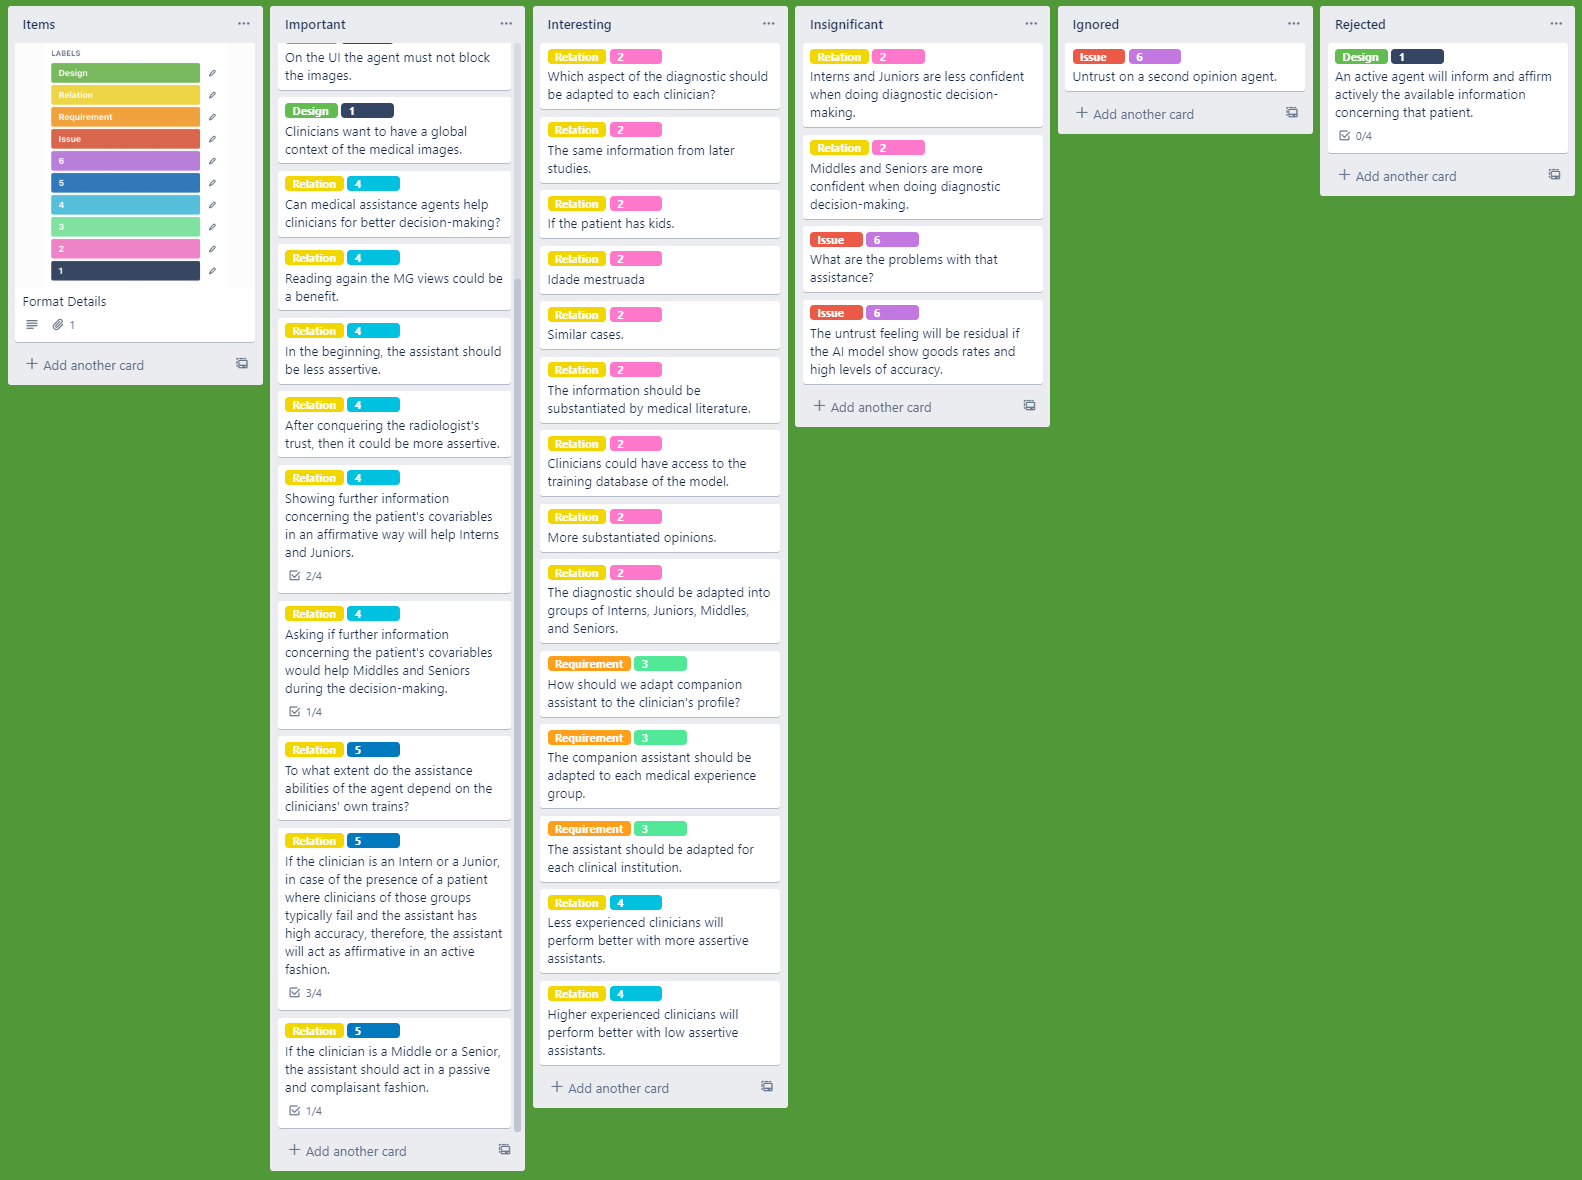
\includegraphics[width=\linewidth]{fig025}
\caption{Resulting affinity diagrams passed to a digital software tool. The overall ideas and features categorization. Each idea and feature has a category ({\it e.g.}, "Items", "Important", "Interesting", "Insignificant", "Ignored" or "Rejected"), so that we can manage the final requirements and development priorities of our assistant agents.}
\label{fig:fig025}
\end{figure}
%%%%%%%%%%%%%%%%%%%%%%%%%%%%%%%%%%%%%%%%%%%%%%%%%%%

As these ideas and functionalities from the clinicians could be relevant for several purposes, it was considered useful to short on a more general level to start with.
As follows, we describe how we clustered the acquired data based in the {\it affinity} of the collected ideas and features.

\subsection{Data Clustering}
\label{sec:sec00504}

As notes are placed, and in moving them around later, they are clustered based in their {\it affinity}, {\it i.e.}, their similarity or relevance to a shared topic.
This leads to the creation of data groups, which are labeled and recursively clustered.
The process repeats until the highest level has only a few groups and the initially unstructured items have been organized bottom-up.
Clusters and then given titles are grouped into more abstract groups, giving rise to general and overarching ideas.
Ideas are then clustered again to identify common issues and potential solutions, ultimately helping to frame the user needs and design problems.